\textbf{These subsections below should be combined and explain how the simulations are stored in root files and which resources that were utilized to extract/read relevant information from these}

\subsection{Dataset Preparation and Storage}
\label{sec:method_processing}

\texttt{ROOT} reading and tensorization are implemented separately from model training. The reader uses the \texttt{uproot} Python package \cite{uproot_software} and jagged arrays to extract the required
collections in chunks, aligns truth contributions to reconstructed hits, and
passes both preprocessed (see \ref{sec:preprocess}) and plain event records to the tensorization step. Tensorization constructs
features, masks, dominant labels and, when requested, fraction and noise
targets. This separation makes the physics definition of a target independent
of the particular neural-network architecture and 
% This is a very important distintiction and I want this formulation preserved "this is a conscious and important design choice." 
this is a conscious and important
design choice. 
Keeping the I/O and tensorization steps separate and contained
also allows new models to be implemented and tested by the user without modifying the data processing.

For repeated training, tensorized events can be written as \texttt{PyTorch}
\texttt{.pt} data rather than being reconstructed from \texttt{ROOT} for every run, to save time and computational resources. The \texttt{TTree} format used in \texttt{ROOT} is optimized for compressed
columnar storage and selective, high-throughput access to individual branches
\cite{root_ttree}. The \texttt{PyTorch} shards therefore contain only the features and
targets required for the \gls{ml} tasks, avoiding an unnecessary conversion of
the complete simulation output.

The resulting pipeline provides a practical path from simulation in the
\gls{ldmxsw} framework built upon \gls{geant4}, where events are stored in \texttt{ROOT} files, to
\gls{ml}-ready shards stored as \texttt{PyTorch} files. The complete workflow is
illustrated in Figure~\ref{fig:data_pipeline}.

A manifest is also output by the reader that records the source inputs, feature
layout, allowed labels, and noise policy. The sharded representation
additionally stores an index of event ranges and supports lazy loading, i.e.\
individual shards are loaded from disk only when their events are requested,
rather than loading the entire dataset into memory.



\subsubsection{Preprocessing of Energy Features from the ECal and TS subdetectors}
\label{sec:preprocess}

The input features that represent energy measurements from the \gls{ecal} and \gls{ts} subdetectors, reconstructed energy of an \gls{ecal} cell hit "\gls{rechit} energy" and the photoelectron readout from the \gls{ts} "pe", are generally not suitable for training in its' raw numerical form. It is common nature for energy measurements
\begin{wrapfigure}{r}{0.50\textwidth}
    \centering
    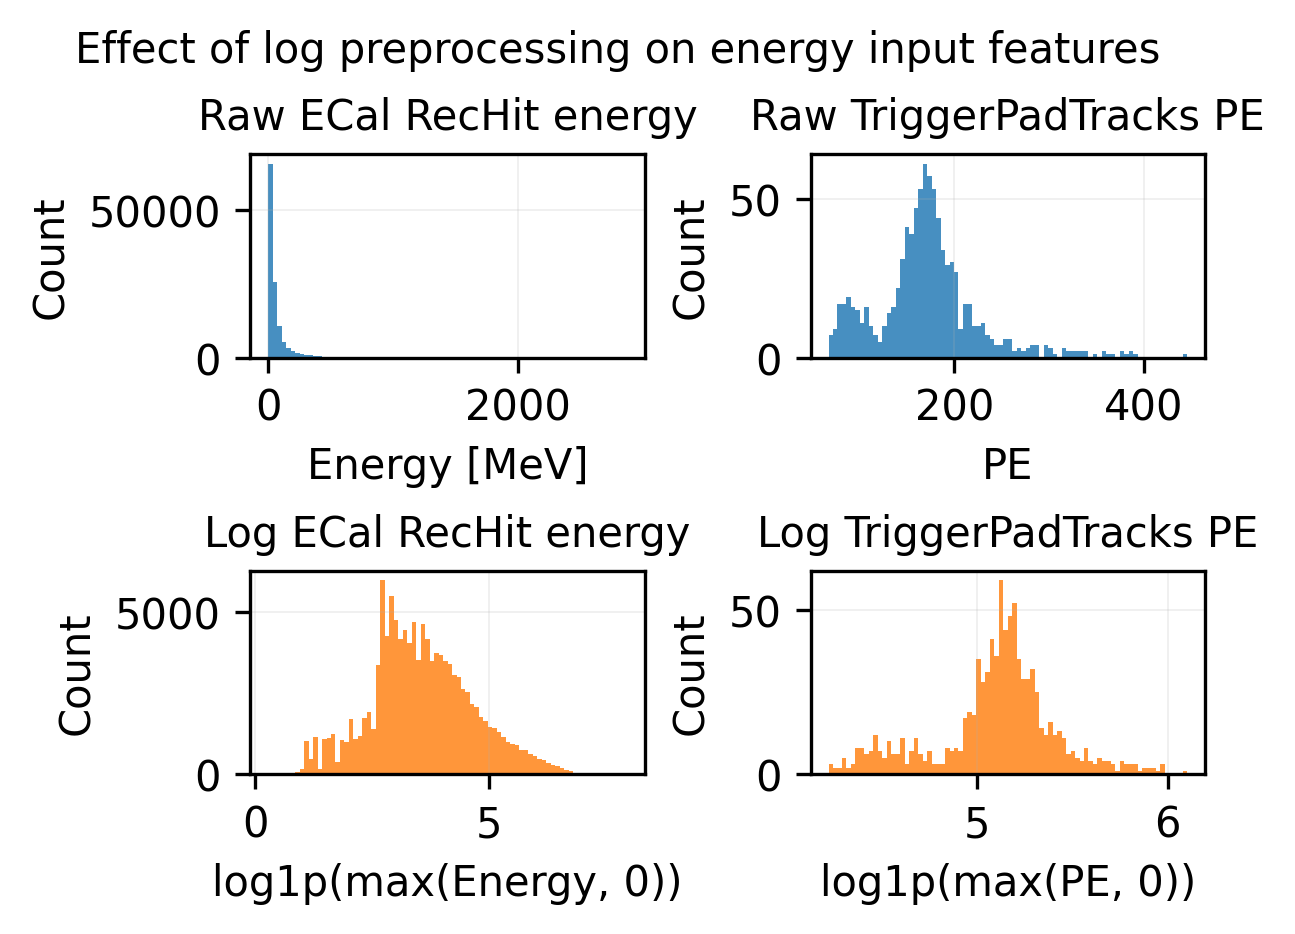
\includegraphics[width=0.48\textwidth]{config/fig/log1p_2x2.png}
    \caption{Histograms showing the distribution of energy values from subdetectors before and after a log transform.}
    \label{fig:skew_and_log}
\end{wrapfigure} 
in this context to have a skewed distributions, i.e a high density in one end of the distribution and a long tail on the other end, and skewed distributions are not ideal for machine learning \cite{lai2024shower}. The energy distributions for both RecHit energy and the pe over the simulated events were by simple inspection by eye confirmed to be right skewed, especially the reconstructed energy from the \gls{ecal}, see figure \ref{fig:skew_and_log}. To attend to this problem these features were put through a standard procedure of a log transform, specifically using the \texttt{log1p()} function from the \texttt{torch} package \cite{pytorch_log1p}. The log transform is suitable to use since energy is inherently non-negative, it compacts the magnitude which eases numerical operations and it preserves ordering, which is the critical piece of information for \gls{ml} models. After the log transform, one can see in figure \ref{fig:skew_and_log} that the differentiation of values in the distribution is enhanced and more ideal for inference and training computations.

In tensorization of the original simulation \texttt{ROOT} files to tensor shards, the energy features are saved after the log transform with the original naming scheme but a copy containing the original raw energy features are also saved with a ''\texttt{\_raw}'' suffix, since the raw values can be 

\subsubsection{Dataset retrieval and split in training}

Events are randomly assigned, with a fixed seed, to training, validation and
test subsets in proportions \(80\%\), \(15\%\) and \(5\%\), respectively.
The normalization statistics, optional class weights and parameter updates
are determined from the training subset only. Validation data are used for
checkpoint selection and optional learning-rate scheduling, while test data
are held for final evaluation.

\subsection{Simulation Data and Data Extraction}


\subsubsection{ROOT Collections}



The input events are simulated with the \gls{geant4}-based \gls{ldmxsw}
framework and stored in a ROOT tree named \texttt{LDMX\_Events}. The
supervised pipeline reads reconstructed \gls{ecal} hits from
\texttt{EcalRecHits\_overlay}. For each reconstructed hit it extracts the
cell identifier, Cartesian position, reconstructed energy and the stored
noise flag. Truth association is obtained from
\texttt{EcalSimHitsOverlay\_overlay}, which contains, per detector cell, the
track identifiers, energy depositions and origin identifiers of the
contributing simulated particles. Reconstructed and simulated hit records are
aligned by detector cell identifier. Thus, the network inputs remain
reconstructed quantities, whereas simulation information is used to construct
training targets.

The context-aware models additionally read
\texttt{TriggerPadTracks\_overlay}. In the implemented pipeline, each such
object contributes its \texttt{centroid} coordinate and its number of
photoelectrons, \texttt{pe}. These objects are treated as context nodes or
tokens: they can influence an \gls{ecal} prediction, but do not receive
hit-origin supervision themselves.

\subsubsection{Overlay Event Samples}

The data-loading and training code supports separate overlay sources marked
by their electron multiplicity. In particular, it accepts two-electron
(\(2e\)) and three-electron (\(3e\)) sources and can combine them in one
processed dataset. The fixed-three-origin development sample is useful for
testing shower assignment, while mixed \(2e\)/\(3e\) data enable the event-level
electron-count task. Since the conclusions drawn from a trained model depend
on the particular selected subset and split, sample sizes and numerical
performance are reported with the corresponding results rather than assumed
in the definition of the method.

\subsection{Supervised Targets}
\label{sec:method_targets}

The principal task covered in this report is originating electron classification. For the baseline models some key simplifications were made that must be clearly stated:

\begin{enumerate}
    \item \textbf{Pile-up level prior} The baseline models are trained exclusively on $2e$ or $3e$ events, indirectly informing the reconstruction model on the number of electrons present in the event (''pile-up level''). This isolates the models assignments to only the originating electron task, but it in a real-world scenario this is not a known fact in prior. The ideal reconstruction model would also be tasked to predict the pile-up level as well, or the baseline reconstruction model should be put in a context where there is another method that predicts the number of electrons before using an originating electron classifier. 
    \item \textbf{Dominant-Contribution Labeling:} Hits in the \gls{ecal} detector can consist of energy contribuition from several electrons in pile up events. This introduces ambiguity in analysis, but also in the design of the reconstruction models of how it should handle this. To simplify, the \gls{ecal} hits with a number of energy contributions more than $1$ are relabeled to only the originating electron with the highest energy contribution. 
    \item \textbf{Noise hits filtration:} In the real experiment, random background noise is expected to occur as hits in the \gls{ecal} detector. Noise is also implemented in the simulations, but to simplify the design and training of the baseline models these noise hits are simply omitted. 
\end{enumerate}

\subsubsection{Dominant-Contribution Hit Labels}

A reconstructed hit may contain simulated energy deposited by more than one
overlaid electron. If \(e_{ij}\) is the energy contribution to reconstructed
hit \(i\) associated with origin \(j\), its hard assignment target is defined
by
\begin{equation}
    y_i^{\mathrm{origin}} =
    \argmax_{j \in \{1,2,3\}} e_{ij}.
    \label{eq:dominant_origin_target}
\end{equation}
The implemented ROOT-to-tensor conversion selects the origin identifier of
the largest deposited-energy contribution and maps accepted physical origin
identifiers \(1,2,3\) to class indices appropriate for the training loss.
This target asks which electron dominates the reconstructed hit; it does not
assert that a hit with contributions from several showers is physically
unmixed.

For the multi-task models, the deposited-energy contributions also define a
soft target,
\begin{equation}
    f_{ij} =
    \frac{e_{ij}}{\sum_k e_{ik}},
    \qquad
    \sum_j f_{ij}=1
\end{equation}
when all retained contributions correspond to the configured electron
origins. Predicting \(f_{ij}\) retains information about hits near an overlap
region that is discarded by the dominant-origin label alone.

\subsubsection{Noise and Canonical Electron Slots}

Hits marked as detector noise are excluded from the maintained hit-origin
baseline comparisons. The advanced slot-model path can instead retain these
hits and assign them to an explicit background class \(0\), with a
background-only fraction target. Noise-labelled hits are not used to
determine the presence or ordering of electron slots.

An origin identifier introduced during overlay is a provenance label rather
than an ordered physical observable: exchanging the identifiers of two
electrons leaves the reconstruction problem unchanged. To remove this
permutation ambiguity, the maintained comparisons use a canonical spatial
target. For each electron present in an event, the mean \(y\)-coordinate of
its selected \gls{ecal} hits is calculated. Electrons are ordered by this
mean coordinate, and their targets are remapped to canonical slots from
lowest to highest \(y\). The same reordering is applied to the fraction
targets. The original origin identifiers are retained in the processed
events for provenance. Other spatial axes are implemented for controlled
studies, while canonical ordering in \(y\) is the standard comparison
configuration because it provides a consistent relation to the available
one-dimensional trigger-pad centroid information.

\subsection{Feature Construction and Event Representation}
\label{sec:method_features}

The ECal-only representation supplies one row
\((x_i,y_i,z_i,E_i)\) for each retained reconstructed hit. The combined
representation places \gls{ecal} hits and trigger-pad-track objects in one
event tensor with the feature layout shown in
Table~\ref{tab:combined_features}. Type-indicator columns identify the
detector collection, while non-applicable continuous fields are zero-filled.
Boolean masks retain which rows correspond to ECal hits and which correspond
to trigger-pad tracks.

\begin{table}[H]
    \centering
    \caption{Implemented feature layout for the combined ECal and
    trigger-pad-track representation.}
    \label{tab:combined_features}
    \begin{tabular}{lll}
        \hline
        Columns & ECal hit row & Trigger-pad-track row \\
        \hline
        \texttt{is\_ecal}, \texttt{is\_tpad} & \(1,0\) & \(0,1\) \\
        \texttt{ecal\_x}, \texttt{ecal\_y}, \texttt{ecal\_z} &
            \(x,y,z\) & \(0,0,0\) \\
        \texttt{ecal\_energy} & \(E\) & \(0\) \\
        \texttt{tpad\_centroid}, \texttt{tpad\_pe} &
            \(0,0\) & \(c,n_{\mathrm{pe}}\) \\
        \hline
    \end{tabular}
\end{table}

All continuous columns in this canonical combined representation are
standardized using means and standard deviations calculated only from the
training split. The fitted statistics are then applied to validation and test
events and stored with the run artifacts. The detector-type indicator columns
are not standardized.

The maintained models process one variable-length event at a time. Several
events are accumulated before one optimizer update, but no fixed maximum
number of detector objects is imposed by the main training pipeline. For
models receiving both detector collections, the \texttt{ecal\_mask} restricts
the hit-level loss and hit-level metrics to \gls{ecal} rows. This distinction
allows trigger-pad-track tokens to provide information without requiring an
artificial hit-origin target for them.




%%%%%%%%%%%%%%%%%%%%%%%%%%%%%%%%%%%%













\subsection{Stuff I want to mention sometime and fit in}


\paragraph{Event energy-weighted accuracy.}
For an event with ECal hits indexed by \(i\), the energy-weighted accuracy is
defined as
\[
A_{\mathrm{energy}}
=
\frac{
    \sum_i E_i\,\mathbb{I}\!\left(\hat{y}_i = y_i\right)
}{
    \sum_i E_i
},
\]
where \(E_i\) is the reconstructed energy of hit \(i\), \(y_i\) is its true
class, \(\hat{y}_i\) is its predicted class, and \(\mathbb{I}(\cdot)\) is the
indicator function. Consequently, correctly classifying a high-energy hit
contributes more than correctly classifying a low-energy hit.

For example, consider two hits with energies \(9\) and \(1\), where only the
hit with energy \(9\) is classified correctly. The ordinary event accuracy is
\[
A_{\mathrm{event}} = \frac{1}{2} = 0.5,
\]
whereas the energy-weighted accuracy is
\[
A_{\mathrm{energy}} = \frac{9}{9+1} = 0.9.
\]

\paragraph{Mean event accuracy.}
The ordinary accuracy of event \(e\) is
\[
A_e
=
\frac{N_{\mathrm{correct},e}}{N_{\mathrm{hits},e}}.
\]
The mean event accuracy is then the arithmetic mean of the individual event
accuracies:
\[
\overline{A}_{\mathrm{event}}
=
\frac{1}{N_{\mathrm{events}}}
\sum_{e=1}^{N_{\mathrm{events}}} A_e.
\]
Thus, every event contributes equally, regardless of how many hits it
contains. This is not an average over the individual electrons.

\paragraph{Hit accuracy.}
The hit accuracy instead pools all hits from all events:
\[
A_{\mathrm{hit}}
=
\frac{
    \sum_e N_{\mathrm{correct},e}
}{
    \sum_e N_{\mathrm{hits},e}
}.
\]
Events containing more hits therefore contribute more strongly to the hit
accuracy. The reported training, validation, and test accuracies use this
pooled hit-level definition.












